\documentclass[11pt,a5paper]{report}
\usepackage[a5paper,total={128mm, 180mm}]{geometry}


\usepackage[dutch]{babel}
\usepackage{graphicx, wrapfig}
\usepackage{amsmath}
\usepackage{bm}
\usepackage{multicol}

\usepackage{cancel}
\usepackage{fancyhdr}
\usepackage{float}
\usepackage{titlesec}
\usepackage{parskip}
\usepackage{caption}
\usepackage{array}
\usepackage{framed}


\titleformat{\section}{\normalfont\Large\bfseries}{\thesection.}{1em}{}
\titleformat{\subsection}{\normalfont\large\bfseries}{\thesubsection.}{1em}{}
\renewcommand{\familydefault}{\sfdefault}

\title{PIDAC Practicumhandleiding \\ \Large Datarepresentaties, Tools en Technieken}
\author{}
\date{}


\begin{document}

\begin{titlepage}
	\raggedright

	{\Huge PIDAC\par}
	{\LARGE Practicumhandleiding\par}
	{\LARGE Naam: \par}
		\vfill
		
	
\includegraphics[width=0.39\textwidth]{images/uvalogo_regular_compact_p_nl.eps}\par\vspace{0cm}	
	{\LARGE Minor Programmeren\par}
	{\LARGE Datarepresentaties, Tools en Technieken\par}

\end{titlepage}
\ 

\vfill
Universiteit van Amsterdam \\
Versie: 3 (08-2025) \\
Auteur: Simon Pauw \\
Geïnspireerd door de syllabus \textit{Digitale Techniek} van Ben Bruidegom \\
Met input van: Edwin Steffens en Puck te Rietmolen

\thispagestyle{empty}

\newpage

\section*{Practicumregels}
\ 
\vfill
\begin{figure}[H]
\centering

\includegraphics[width=0.2\textwidth]{./images/warning.png}
\end{figure}

\textbf{Wees voorzichtig met het gebruik van de PIDAC-modules.} Deze modules worden niet meer geproduceerd en de losse onderdelen zijn vaak niet meer verkrijgbaar. Reparatie is meestal niet mogelijk. Houd je daarom aan de volgende regels: \\

\textbf{Laat modules niet rondslingeren.} \\

Pak een module direct uit de doos en plaats hem meteen op het experimenteerbord. \\

Let erop dat je de pinnen aan de achterkant niet buigt of breekt bij het plaatsen. \\ 

Leg modules die je niet meer nodig hebt terug in de doos waar ze vandaan kwamen. \\

Trek stroomdraadjes eruit bij de stekker en niet aan de draad zelf. \\

\vfill


\newpage
\ 
\chapter*{\centering Week 1}
\newpage

\section*{Deel 1. Schakelingen en notaties}

Je hebt maar een beperkt aantal logische poorten nodig om elke mogelijke schakeling te kunnen bouwen. Het doel van dit deel is om vertrouwd te raken met deze poorten en de manieren waarop we hiermee schakelingen kunnen bouwen. Je leert ook hoe je schakelingen symbolisch kunt beschrijven.

\subsection*{Logische poorten}

De NAND-poort heeft het volgende gedrag: op de uitgang staat 5 volt, tenzij beide ingangen 5 volt ontvangen. Dan staat er 0 volt op de uitgang. Je kunt dit zelf testen met een woordgever en een indicator.

\begin{figure}[H]
\centering
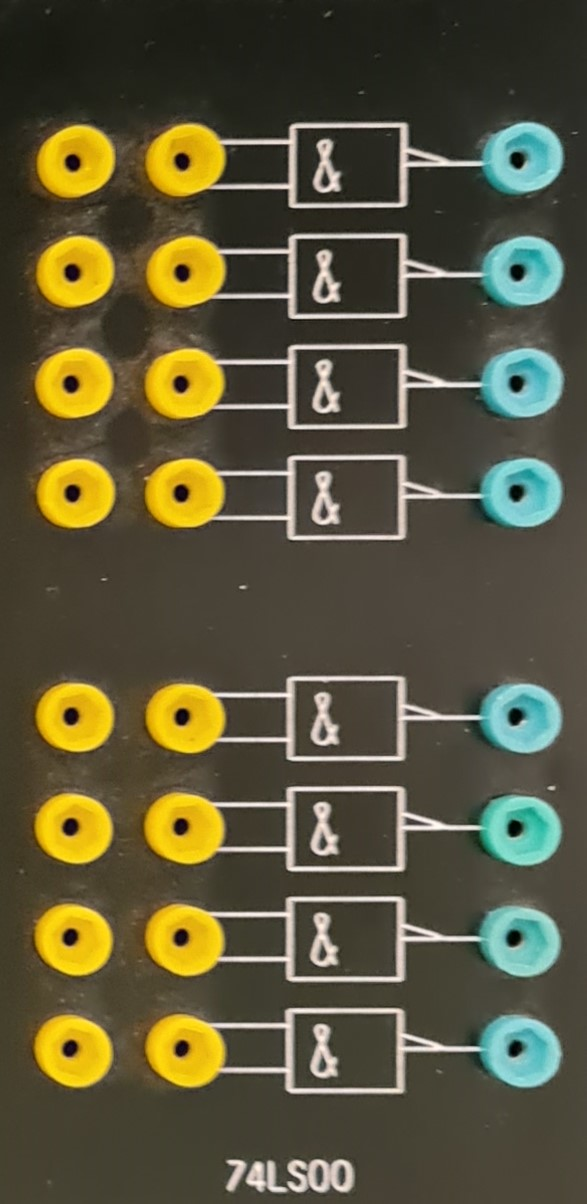
\includegraphics[width=0.255\textwidth]{./images/2nand.jpg}
\hspace{0.05\textwidth}
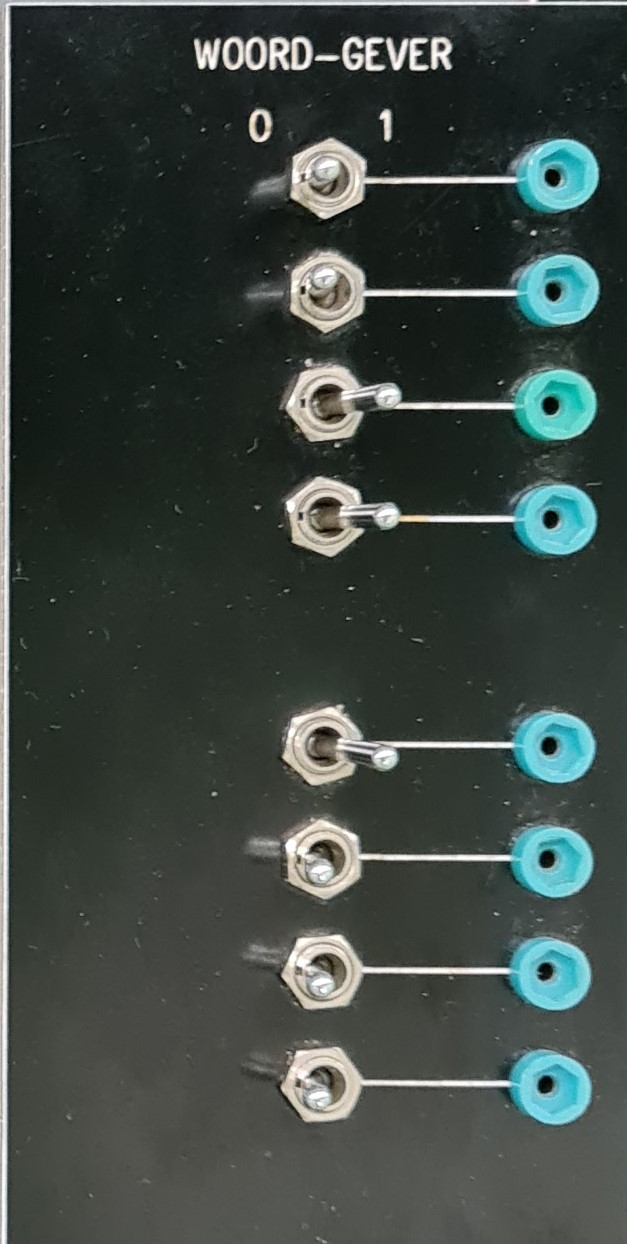
\includegraphics[width=0.263\textwidth]{./images/woordgever.jpg}
\hspace{0.05\textwidth}
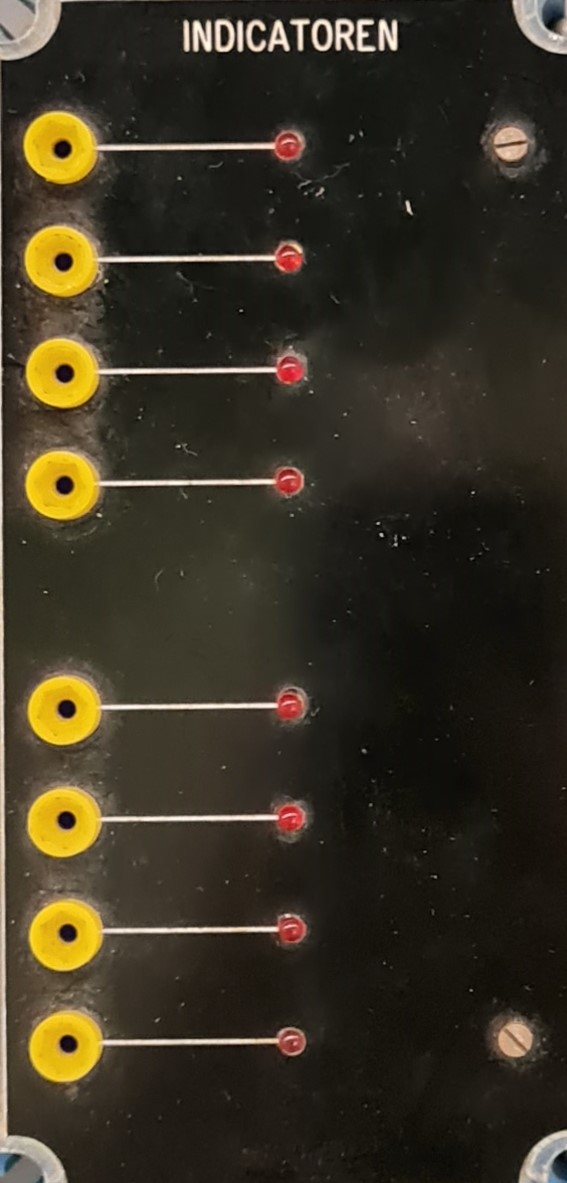
\includegraphics[width=0.25\textwidth]{./images/indicatoren.jpg}
\caption*{PIDAC Modules (vlnr): NAND, Woordgever, Indicator}
\end{figure}




\begin{framed}
\textbf{Opdracht 1.1} \textbf{Lees de practicumregels goed door voordat je begint.} 

Bouw een schakeling om te testeb of de beschrijving van de NAND-poort klopt. (Nodig: NAND-module, woordgevermodule, indicatormodule en drie draadjes.)


\end{framed} 

\section*{Eentjes en nulletjes}

Computers werken met eentjes en nulletjes. Elke poort kan in twee toestanden zijn: 5 volt (hoog, ofwel 1) of 0 volt (laag, ofwel 0).

Niet alle digitale schakelingen werken op 5 volt; sommige gebruiken bijvoorbeeld 3,3 volt als hoog. Maar ongeacht het exacte voltage zijn er altijd twee toestanden: hoog en laag.

\section*{Notatie}

\begin{minipage}[t]{0.7\textwidth}
Het gedrag van een logische poort wordt beschreven door een waarheidstabel. Hiernaast zie je de waarheidstabel voor een NAND-poort met twee ingangen $y$ en $z$ en uitgang $Q$.
\end{minipage}%
\hfill
\begin{minipage}[t]{0.2\textwidth}
\vspace*{-1em}
\(
\begin{array}{cc|c}
y & z & Q \\
\hline
0 & 0 & 1 \\
0 & 1 & 1 \\
1 & 0 & 1 \\
1 & 1 & 0 \\
\end{array}
\)
\end{minipage}\\



\begin{minipage}[t]{0.7\textwidth}
De symbolische notatie van een NAND-poort, zoals wij deze verder in dit document zullen gebruiken:
\end{minipage}%
\hfill
\begin{minipage}[t]{0.2\textwidth}
\vspace*{-1em}
\centering
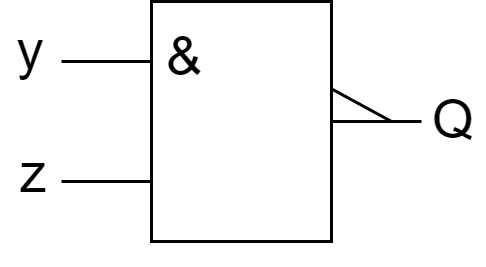
\includegraphics[width=1.0\textwidth]{./images/NAND.png}
\end{minipage}\\



\begin{minipage}[t]{0.7\textwidth}
Er zijn verschillende notatiesystemen voor logische poorten, je zal voor de NAND-poort ook vaak dit alternatief tegenkomen:
\end{minipage}%
\hfill
\begin{minipage}[t]{0.2\textwidth}
\vspace*{-1em}
\centering

\includegraphics[width=1.0\textwidth]{./images/dist_NAND.png}
\end{minipage}\\


\begin{minipage}[t]{0.7\textwidth}
Complexere schakelingen kunnen worden opgebouwd door poorten met elkaar te verbinden:
\end{minipage}%
\hfill
\begin{minipage}[t]{0.27\textwidth}
\vspace*{-1em}
\centering
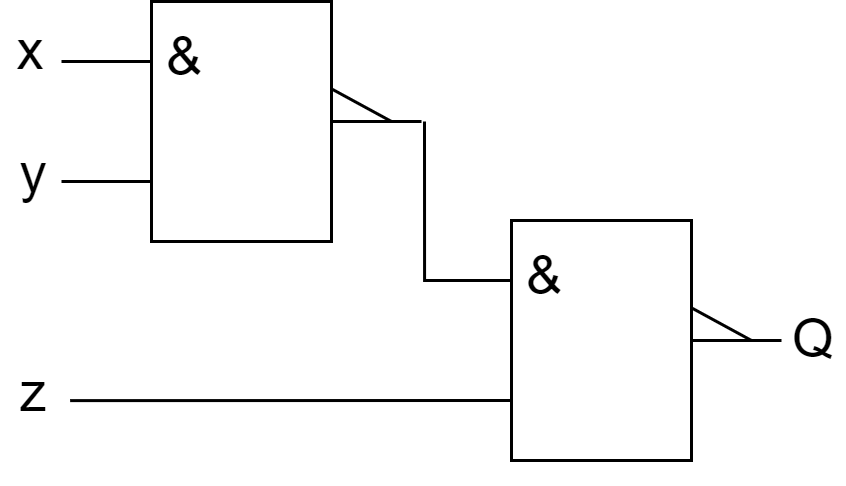
\includegraphics[width=1.0\textwidth]{./images/opdracht1_2.png}
\end{minipage}\\

\begin{framed}
\textbf{Opdracht 1.2} Nodig: twee NAND-poorten, een woordgever, een indicator en vijf draadjes. Bouw de bovenstaande (complexe) schakeling en vul de waarheidstabel op het antwoordblad in.
\end{framed}

\newpage

\section*{Veelvoorkomende poorten}
\newcommand{\portwidth}{0.2\textwidth}
\begin{table}[H]
\centering
\begin{tabular}{|>{\centering\arraybackslash}m{2cm}|>{\vspace{3pt}\centering\arraybackslash}m{3cm}|>{\vspace{4pt}\centering\arraybackslash}m{3cm}|>{\vspace{3pt}\centering\arraybackslash}m{2.2cm}|}
\hline
Poort & Rechthoekige notatie & Alternatieve notatie & Waarheidstabel \\
\hline
AND & 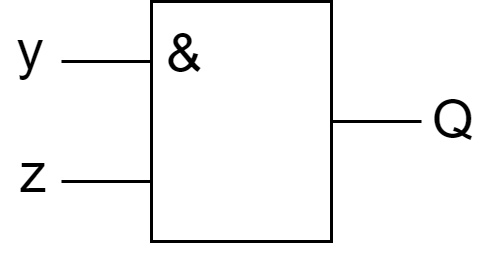
\includegraphics[width=\portwidth]{./images/AND.png} & 
\includegraphics[width=\portwidth]{./images/dist_AND.png} &
\raisebox{0.8\height}{$
\begin{array}{cc|c}
y & z & Q \\
\hline
0 & 0 & 0 \\
0 & 1 & 0 \\
1 & 0 & 0 \\
1 & 1 & 1 \\
\end{array}$}\\
\hline
OR & 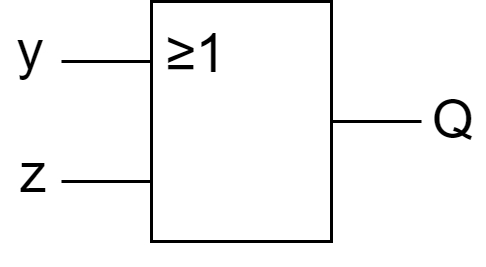
\includegraphics[width=\portwidth]{./images/OR.png} & 
\includegraphics[width=\portwidth]{./images/dist_OR.png} &
\raisebox{0.8\height}{$
\begin{array}{cc|c}
y & z & Q \\
\hline
0 & 0 & 0 \\
0 & 1 & 1 \\
1 & 0 & 1 \\
1 & 1 & 1 \\
\end{array}
$} \\
\hline
XOR & 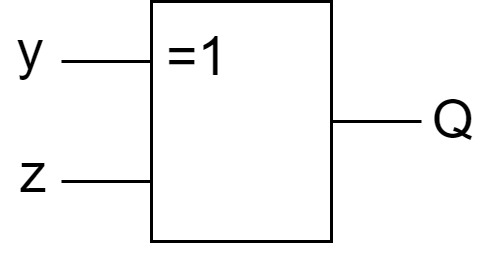
\includegraphics[width=\portwidth]{./images/XOR.png} & 
\includegraphics[width=\portwidth]{./images/dist_XOR.png} &
\raisebox{0.8\height}{$
\begin{array}{cc|c}
y & z & Q \\
\hline
0 & 0 & 0 \\
0 & 1 & 1 \\
1 & 0 & 1 \\
1 & 1 & 0 \\
\end{array}
$} \\
\hline
Inverter & \includegraphics[width=\portwidth]{./images/Inverter.png} & 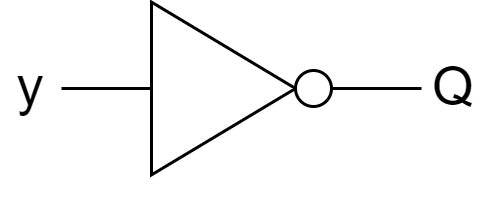
\includegraphics[width=\portwidth]{./images/dist_inverter.png} &
\raisebox{0.7\height}{$
\begin{array}{c|c}
y & Q \\
\hline
 0 & 1 \\
 1 & 0 \\
\end{array}
$} \\
\hline
NAND & 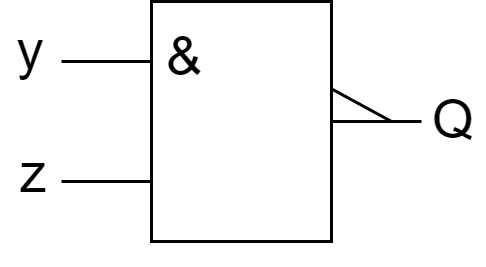
\includegraphics[width=\portwidth]{./images/NAND.png} & 
\includegraphics[width=\portwidth]{./images/dist_NAND.png} & 
\raisebox{0.8\height}{$
\begin{array}{cc|c}
y & z & Q \\
\hline
0 & 0 & 1 \\
0 & 1 & 1 \\
1 & 0 & 1 \\
1 & 1 & 0 \\
\end{array}
$} \\
\hline
NOR & 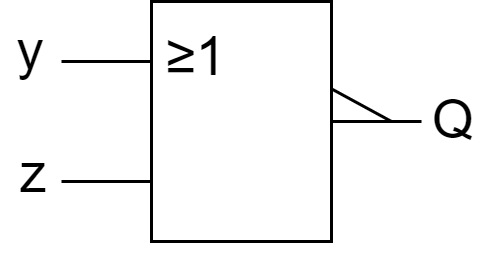
\includegraphics[width=\portwidth]{./images/NOR.png} &
\includegraphics[width=\portwidth]{./images/dist_NOR.png}&
\raisebox{0.8\height}{$
\begin{array}{cc|c}
y & z & Q \\
\hline
0 & 0 & 1 \\
0 & 1 & 0 \\
1 & 0 & 0 \\
1 & 1 & 0 \\
\end{array}
$} \\

\hline
\end{tabular}
\caption*{Overzicht van veelvoorkomende logische poorten}
\end{table}

\section*{Meerdere ingangen}

De bovenstaande poorten hebben allemaal twee ingangen (behalve de inverter), maar in principe kunnen dat er ook meer zijn. Het PIDAC-systeem bevat bijvoorbeeld ook NAND-poorten met vier ingangen. De schematische weergave en waarheidstabel van een NAND-poort met vier ingangen ziet er zo uit:

\begin{table}[H]
\centering
\begin{tabular}{|>{\centering\arraybackslash}m{3.2cm}|>{\centering\arraybackslash}m{3cm}|>{\centering\arraybackslash}m{3cm}|}
\hline
Module & Symbool & Waarheidstabel \\ \hline
\vspace{0.3cm}
\raisebox{-0.5\height}{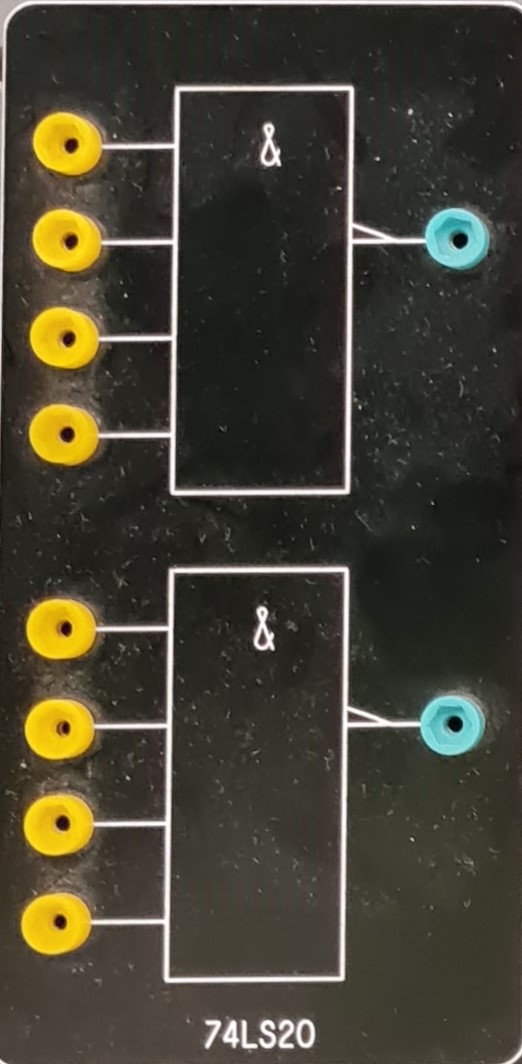
\includegraphics[width=0.25\textwidth]{./images/4nand.jpg}} &
\vspace{2cm}\raisebox{-0.5\height}{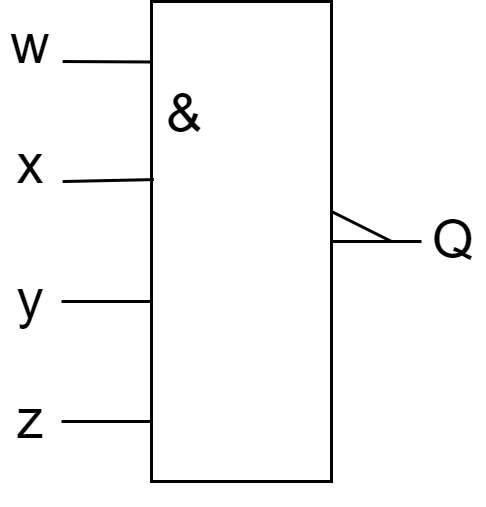
\includegraphics[width=0.2\textwidth]{./images/NAND4.png}} &
\vspace{0.3cm}
\parbox[c]{3cm}{\centering \small
$
\begin{array}{cccc|c}
w & x & y & z & Q \\
\hline
0 & 0 & 0 & 0 & 1 \\
0 & 0 & 0 & 1 & 1 \\
0 & 0 & 1 & 0 & 1 \\
0 & 0 & 1 & 1 & 1 \\
0 & 1 & 0 & 0 & 1 \\
0 & 1 & 0 & 1 & 1 \\
0 & 1 & 1 & 0 & 1 \\
0 & 1 & 1 & 1 & 1 \\
1 & 0 & 0 & 0 & 1 \\
1 & 0 & 0 & 1 & 1 \\
1 & 0 & 1 & 0 & 1 \\
1 & 0 & 1 & 1 & 1 \\
1 & 1 & 0 & 0 & 1 \\
1 & 1 & 0 & 1 & 1 \\
1 & 1 & 1 & 0 & 1 \\
1 & 1 & 1 & 1 & 0 \\
\end{array}
$
}
\\
&&\\
\hline
\end{tabular}
\end{table}



\begin{framed}
\textbf{Opdracht 1.3} Nodig: een module met NAND-poorten met vier ingangen, een woordgevermodule, een indicatormodule en vijf draadjes.

Experimenteer met de NAND-poort. Ga na of de bovenstaande tabel klopt. Wat gebeurt er als een ingang nergens op is aangesloten?
\end{framed}

\newpage
\section*{Poorten samenstellen}



\begin{minipage}[t]{0.55\textwidth}
In principe is de bovenstaande verzameling poorten redundant. Dat wil zeggen, je kunt alle poorten maken met een combinatie van andere poorten. 
\\

Bijvoorbeeld, het schema rechtsboven heeft hetzelfde gedrag als een AND-poort.

We kunnen dit zien aan de hand van de bijbehorende waarheidstabel.
\end{minipage}%
\hfill
\begin{minipage}[t]{0.43\textwidth}
\vspace*{-1em}

\raggedright
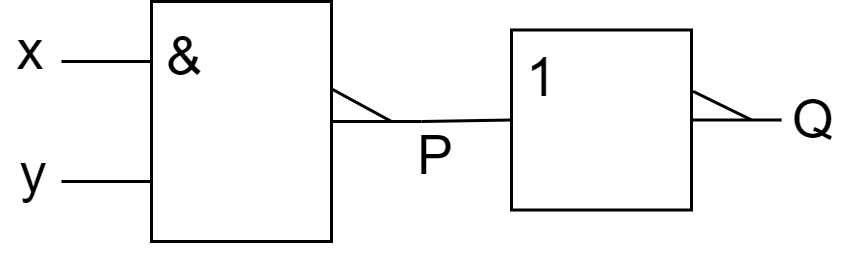
\includegraphics[width=1.0\textwidth]{./images/nand_inverter.png}

\[
\begin{array}{cc|c|c}
x & y & P & Q \\
\hline
0 & 0 & 1 & 0 \\
0 & 1 & 1 & 0 \\
1 & 0 & 1 & 0 \\
1 & 1 & 0 & 1 \\
\end{array}
\]
\end{minipage}\\

\begin{framed}
\textbf{Opdracht 1.4} Je kunt een NAND-poort als inverter gebruiken. Maak een schakeling die dat doet. Gebruik een woordgever en een indicator om je schakeling te testen. Teken het schema op het antwoordformulier en maak een waarheidstabel om te verifiëren dat het klopt.
\end{framed}

\begin{framed}
\begin{minipage}[t]{0.55\textwidth}
\textbf{Opdracht 1.5}  Bouw het schema hiernaast na. Maak een waarheidstabel op je antwoordformulier. Met welke logische poort komt deze schakeling overeen?

Tip: Er zijn geen inverters in PIDAC, maar daar kan je dus NAND-poorten voor gebruiken.
\end{minipage}%
\hfill
\begin{minipage}[t]{0.43\textwidth}
\vspace*{0em}
\centering
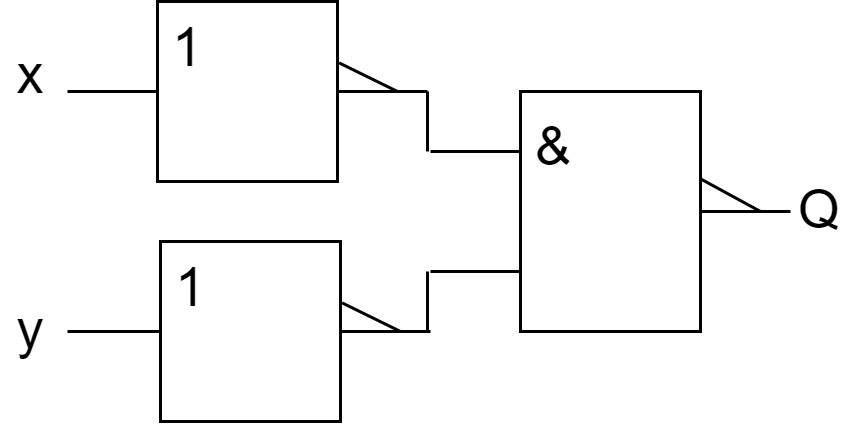
\includegraphics[width=1.0\textwidth]{./images/opdracht1_5.png}
\end{minipage}\\



\end{framed}


\begin{framed}
\textbf{Opdracht 1.6} Maak een schakeling die het gedrag van een NAND-poort met drie ingangen nabootst. Gebruik twee NAND-poorten met twee ingangen en een inverter. Gebruik een woordgever en een indicator om je schakeling te testen. Teken het schema op het antwoordformulier en maak een waarheidstabel om te verifiëren dat het klopt.

\textit{Tip: je kunt een inverter (of NAND) en een NAND-poort gebruiken om een AND-poort te maken. Vervolgens kun je die AND-poort en een NAND-poort combineren tot een NAND-poort met drie ingangen.}
\end{framed}

\newpage
\begin{framed}
\textbf{Opdracht 1.7} Bouw het onderstaande schema na:

\begin{figure}[H]
\centering
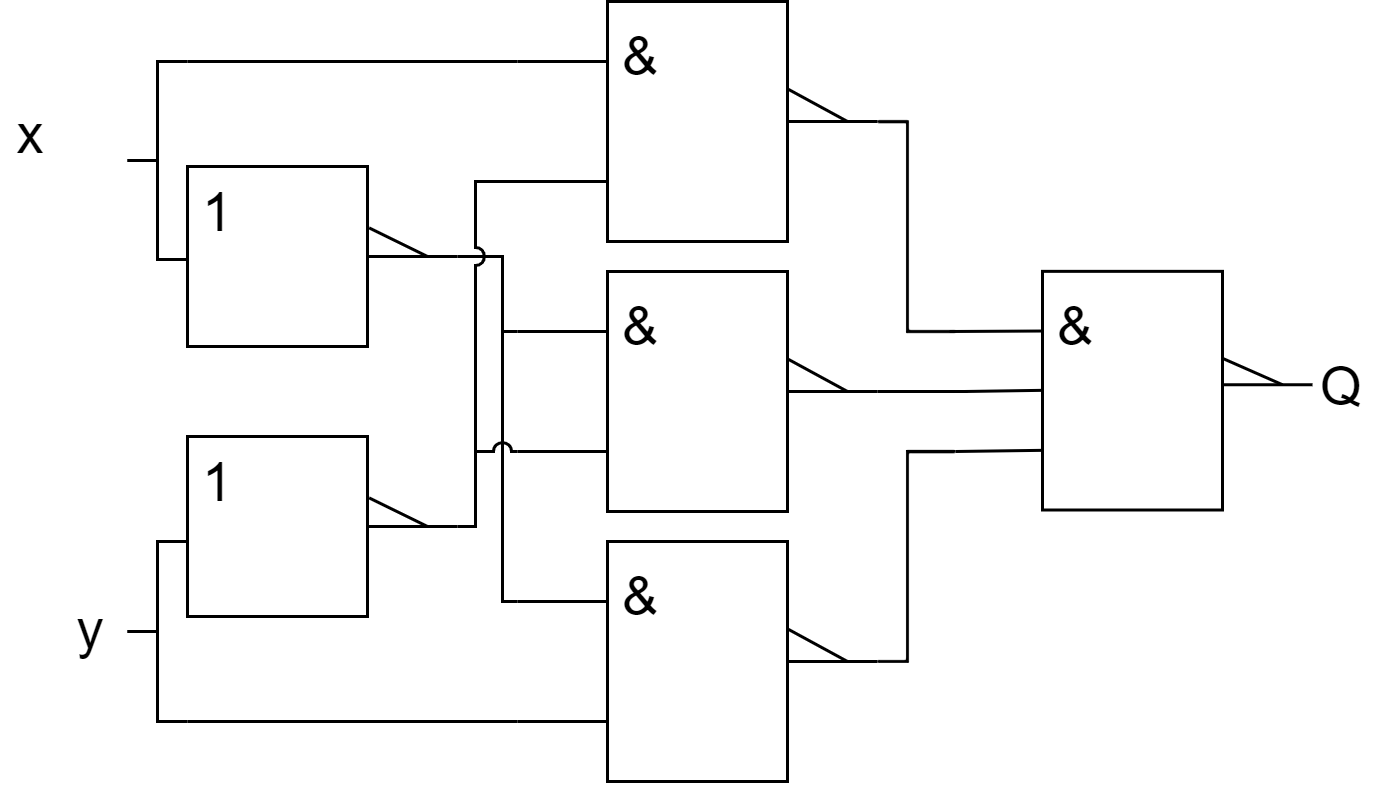
\includegraphics[width=0.65\textwidth]{./images/opdracht1_7.png}
\end{figure}

\textit{De verbindingen van de onderste inverter naar de bovenste twee NAND-poorten bevatten boogjes. Deze geven aan dat de betreffende verbinding een andere kruist zonder ermee verbonden te zijn:}

\begin{figure}[H]
\centering
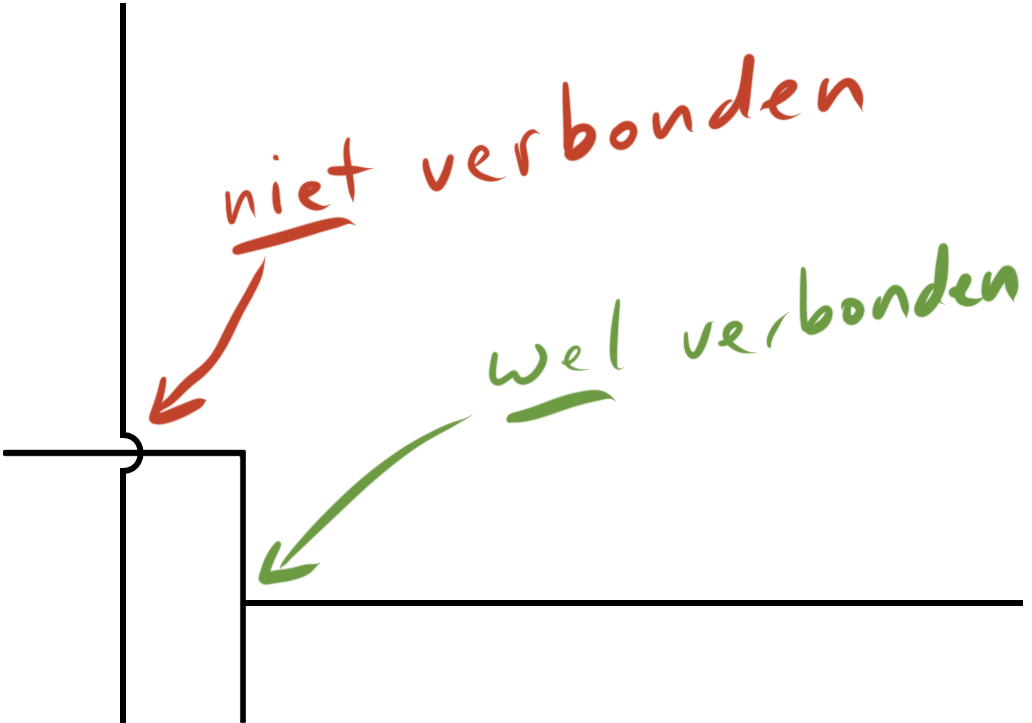
\includegraphics[width=0.4\textwidth]{./images/boogjes.png}
\end{figure}

Maak een waarheidstabel op je antwoordformulier. Vereenvoudig daarna de schakeling. Dat wil zeggen: maak een schakeling die minder poorten gebruikt, maar hetzelfde doet. Teken het schema op je antwoordformulier.

\textit{Voor deze schakeling heb je een NAND-poort met drie ingangen nodig. Er is geen PIDAC-module die zo'n poort heeft, maar je kunt hiervoor een NAND-poort met vier ingangen gebruiken.}
\end{framed}

\begin{framed}
\textbf{Aftekenen!} Laat opdrachten 1.1 - 1.7 aftekenen.
\end{framed}

\section*{Boole-notatie}

Het bouwen van simpele schakelingen kan vaak op basis van intuïtie en uitproberen. Maar bij complexere schakelingen werkt dat niet meer. Daarvoor gebruiken we Boole-algebra. Boole-algebra is in 1854 ontwikkeld door George Boole.

\textit{Als je ervaring hebt met propositielogica, zal Boole-algebra je bekend voorkomen. Het is namelijk equivalent — alleen de notatie verschilt.}

We duiken deze week nog niet volledig in de algebra, maar we leren hoe je Boole-notatie kunt gebruiken om schakelschema's te beschrijven.




\begin{minipage}[t]{0.7\textwidth}
Voor een OR-poort gebruiken we bijvoorbeeld het symbool $\textbf{+}$. Dus het schema hiernaast schrijven we als: $\bm{Q = y + z}$
\end{minipage}%
\hfill
\begin{minipage}[t]{0.27\textwidth}
\vspace*{-1em}
\centering
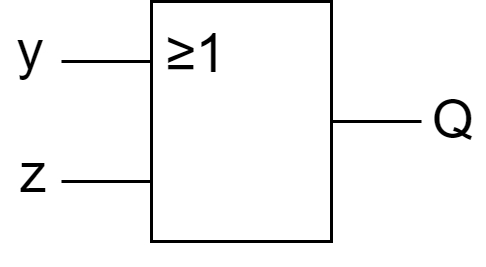
\includegraphics[width=1.0\textwidth]{./images/OR.png}
\end{minipage}\\



Hieronder een overzicht van de notatie van de verschillende poorten:

\begin{table}[H]
\centering
\begin{tabular}{|>{\centering\arraybackslash}m{3cm}|>{\centering\arraybackslash}m{3cm}|>{\vspace{4pt}\centering\arraybackslash}m{3cm}|}
\hline
Poort & Boole-notatie & Schema \\
\hline
OR & $Q = y + z$ & 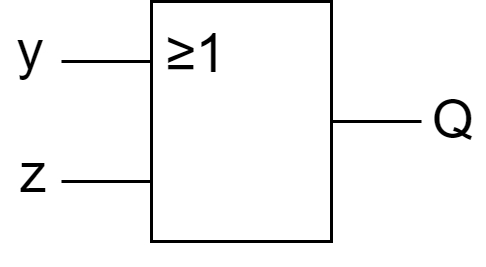
\includegraphics[width=\portwidth]{./images/OR.png} \\ \hline
AND & $Q = y \cdot z$ & 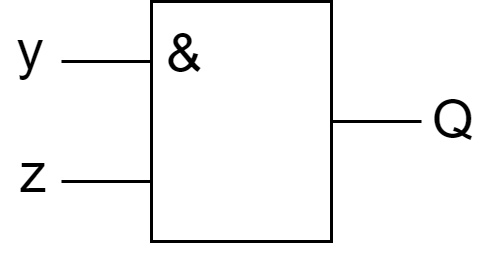
\includegraphics[width=\portwidth]{./images/AND.png} \\ \hline
Inverter & $Q = \overline{y}$ & 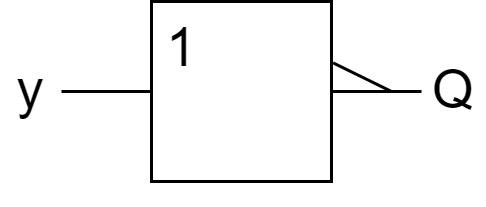
\includegraphics[width=\portwidth]{./images/inverter.png} \\ \hline
XOR & $Q = y \oplus z$ & 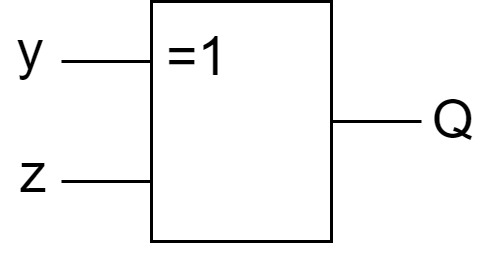
\includegraphics[width=\portwidth]{./images/XOR.png} \\ 
\hline
\end{tabular}
\end{table}

Let op: je hebt het symbool $\oplus$ strikt genomen niet nodig; je kunt XOR ook herschrijven met behulp van $\cdot$, $+$ en $\overline{\phantom{a}}$.

\subsection*{Gebruik Boole-notatie}

We kunnen ook NAND- en NOR-poorten beschrijven met een combinatie van operatoren:

\begin{table}[H]
\centering
\begin{tabular}{|>{\centering\arraybackslash}m{3cm}|>{\centering\arraybackslash}m{3cm}|>{\vspace{4pt}\centering\arraybackslash}m{3cm}|}
\hline
Poort & Boole-notatie & Schema \\
\hline
NAND & $Q = \overline{y \cdot z}$ & 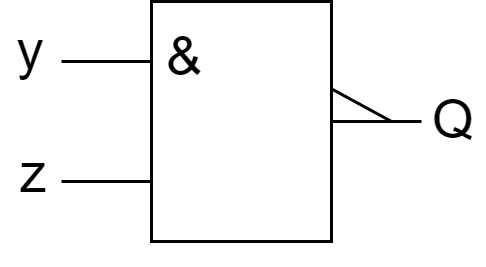
\includegraphics[width=\portwidth]{./images/NAND.png} \\ \hline
NOR & $Q = \overline{y + z}$ & 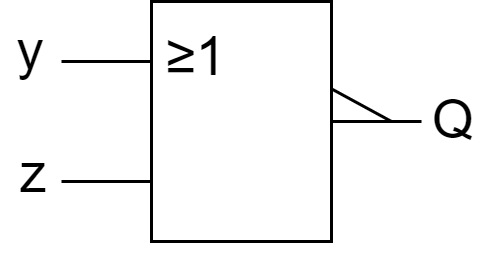
\includegraphics[width=\portwidth]{./images/NOR.png} \\
\hline
\end{tabular}
\end{table}

\vspace{-1.5em}
\subsection*{Complexe schakelingen}

\begin{minipage}[t]{0.6\textwidth}
Complexe schakelingen kunnen we beschrijven met een combinatie van operatoren. Bijvoorbeeld, de schakeling hiernaast schrijven we als: 

\( Q = x \cdot (y + z) \)
\end{minipage}%
\hfill
\begin{minipage}[t]{0.37\textwidth}
\vspace*{-1em}
\centering
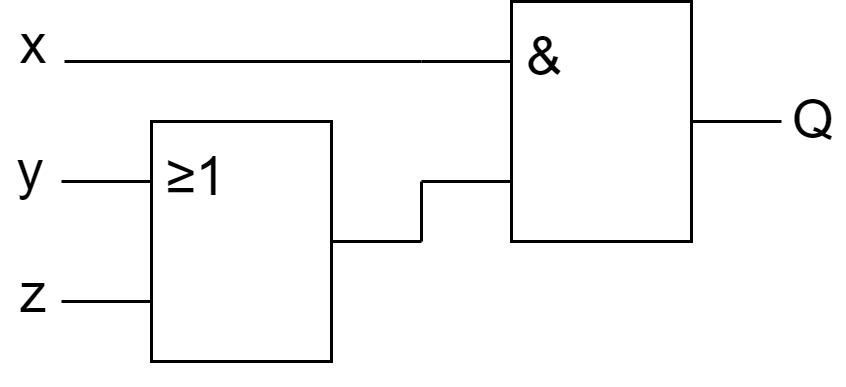
\includegraphics[width=1.0\textwidth]{./images/or_and.png}
\end{minipage}\\


\begin{minipage}[t]{0.6\textwidth}
Een andere voorbeeld, voor de schakeling hiernaast is de expressie:  

\( Q = x + \overline{y \cdot z} \)
\end{minipage}%
\hfill
\begin{minipage}[t]{0.37\textwidth}
\vspace*{-1em}
\centering
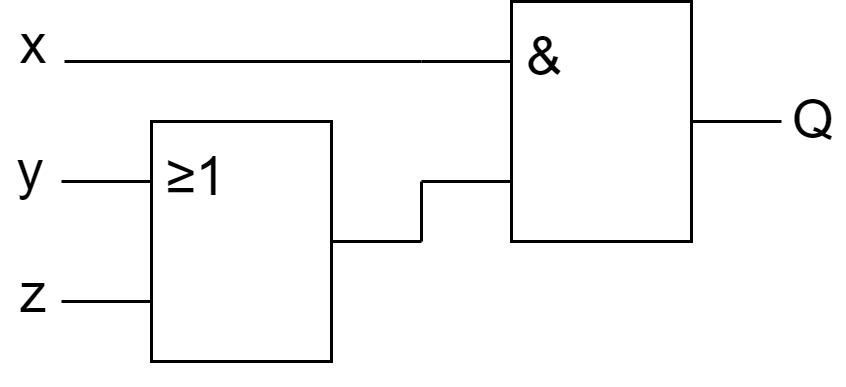
\includegraphics[width=1.0\textwidth]{./images/or_and.png}
\end{minipage}\\

\vspace{-1.5em}
\subsection*{Operatorvolgorde}
Bij Boole-algebra zijn er net als in de wiskunde voorrangsregels regels voor operatoren. Als er geen haakjes staan, gelden de volgende voorrangsregels:
\begin{enumerate}
\item {\bf Negatie} ($\overline{a}$) heeft altijd voorrang.
\item {\bf AND} ($a \cdot b$) komt na negatie maar voor OR.
\item {\bf OR} ($a + b$) en eventueel XOR  ($a \oplus b$) komen als laatste.
\item Bij gelijke operatoren wordt van links naar rechts geëvalueerd.
\end{enumerate}

Bijvoorbeeld, bij  $a + b \cdot c$, evalueren we eerst $b \cdot c$ een daarna pas $a\ +$. \\ \\


\begin{framed}
\textbf{Opdracht 1.8} Bekijk de expressie: \( Q = \overline{\overline{y} \cdot z} \)

Teken het bijbehorende schema, bouw het na en maak een waarheidstabel.
\end{framed}

\begin{framed}
\textbf{Opdracht 1.9} Bekijk de expressie: \( Q = \overline{(a \oplus b) \cdot c} \)

Teken het bijbehorende schema, bouw het na en maak een waarheidstabel.
\end{framed}

\begin{framed}
\textbf{Opdracht 1.10} Bekijk de expressie: \( Q = \overline{\overline{\overline{p}\cdot \overline{q}} \cdot \overline{p \cdot q}} \)

Teken het bijbehorende schema, bouw het na en maak een waarheidstabel.
\end{framed}

\begin{framed}
\textbf{Aftekenen!} Laat opdrachten 1.8 - 1.10 aftekenen.
\end{framed}

\section*{Boole-expressies evalueren}

Je kunt aan de hand van Boole-expressies direct een waarheidstabel opstellen, zonder de schakeling eerst te bouwen. Voor eenvoudige expressies zoals $Q = y + z$, $Q = y \cdot z$ en $Q = \overline{y}$ kun je de waarheidstabellen van de poorten raadplegen (zie de cheatsheet).

Voor complexere expressies vul je gewoon $1$ of $0$ in voor de variabelen en kijk je wat er uitkomt. Neem bijvoorbeeld $Q = \overline{y + z}$. Dit is de expressie van een NOR-poort.

Wat gebeurt er als $y = 1$ en $z = 0$?
\[
Q = \overline{y + z} = \overline{1 + 0} = \overline{1} = 0
\]

Als je dit alle combinaties van $y$ en $z$ doet, krijg je de volgende tabel:
\[
\begin{array}{cc|c}
y & z & Q \\
\hline
0 & 0 & 1 \\
0 & 1 & 0 \\
1 & 0 & 0 \\
1 & 1 & 0 \\
\end{array}
\]

\begin{framed}
\textbf{Opdracht 1.11} We hebben een schakeling gegeven door:
\(
Q = \overline{v \cdot \overline{w}} \oplus p
\)

Beredeneer de waarheidstabel. Als je klaar bent, teken het schema, bouw het en controleer of je waarheidstabel klopt.
\end{framed}

\begin{framed}
\textbf{Opdracht 1.12} We hebben een schakeling gegeven door:
\(
Q = \overline{\overline{a} + b} + c
\)

Beredeneer de waarheidstabel voor deze schakeling.
\end{framed}

\begin{framed} 
\textbf{Opdracht 1.13} NAND-poorten hebben de handige eigenschap dat je er elke andere poort mee kunt bouwen. Ontwerp een schakeling van alleen NAND-poorten die zich gedraagt als een AND-poort. Teken het schema in je antwoordformulier.
\end{framed}

\begin{framed}
\textbf{Aftekenen!} Laat opdrachten 1.11 - 1.13 aftekenen.
\end{framed}

\newpage
\begin{framed}
\textbf{Opdracht 1.14}

Een veelgebruikte schakeling is de dataselector (multiplexer). Stel je een systeem voor met twee datasignalen en een digitale selectielijn. Afhankelijk van de waarde van de selectielijn gaat het ene of het andere signaal door.

\begin{figure}[H]
\centering
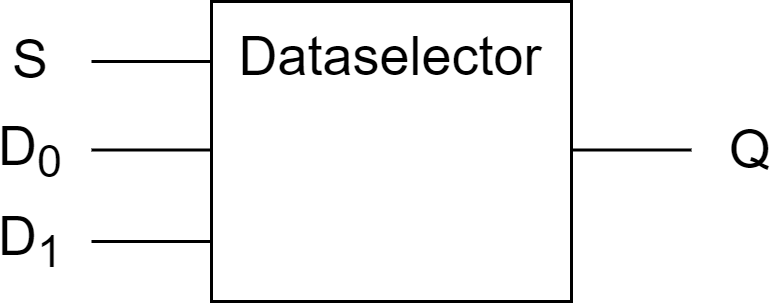
\includegraphics[width=0.35\textwidth]{./images/dataselector.png}
\end{figure}

Inputs: $D_0$, $D_1$, $S$ (select). Output: $Q$

\[
\begin{array}{ccc|c}
S & D_0 & D_1 & Q \\
\hline
0 & d_0 & d_1 & d_0 \\
1 & d_0 & d_1 & d_1
\end{array}
\]

Volledig uitgewerkt:
\[
\begin{array}{ccc|c}
S & D_0 & D_1 & Q \\
\hline
0 & 0 & 0 & 0 \\
0 & 0 & 1 & 0 \\
0 & 1 & 0 & 1 \\
0 & 1 & 1 & 1 \\
1 & 0 & 0 & 0 \\
1 & 0 & 1 & 1 \\
1 & 1 & 0 & 0 \\
1 & 1 & 1 & 1 \\
\end{array}
\]

Ontwerp \textbf{en bouw} een schakeling voor deze tabel. 

Dit kan een flinke puzzel zijn, vraag gerust om hulp van de docent of medestudenten.
\end{framed}

\begin{framed}
\textbf{Aftekenen!} Laat opdracht 1.14 aftekenen.
\end{framed}

\newpage
\section*{Opmerkingen}

\subsection*{Relatie met programmeertalen}

De logica is in programmeertalen is direct gebaseerd op Boole-algebra. Je kan de besproken operatoren dus ook direct terugvinden in verschillende programmeertalen. De notatie is alleen net anders. Bijvoorbeeld:
\begin{itemize}
    \item In plaats van $1$ en $0$ zie je vaak \verb|true| en \verb|false|
    \item $a + b$ wordt \verb/a || b/ in C, of \verb|a or b| in Python
    \item $a \cdot b$ wordt \verb|a && b| in C, of \verb|a and b| in Python
    \item $\overline{a}$ wordt \verb|!a| in C, of \verb|not a| in Python
\end{itemize}

\subsection*{Relatie met propositielogica}

Propositielogica is hetzelfde als Boole-algebra, alleen worden er conventioneel andere symbolen gebruikt:
\begin{itemize}
    \item $1$ en $0$ komen overeen met $\top$ (waar) en $\bot$ (onwaar)
    \item $a + b$ wordt $a \lor b$
    \item $a \cdot b$ wordt $a \land b$
    \item $\overline{a}$ wordt $\neg a$
\end{itemize}



\newpage
\ 
\newpage
\chapter*{\centering Week 2}
\newpage

\section*{Boolealgebra: de kracht van abstractie}

In deze sessie leer je hoe je Boole-algebra kunt gebruiken om schakelingen te ontwerpen. In de vorige sessie heb je geleerd wat het verband is tussen een Boole-expressie en een schakeling. De kracht van Boole-algebra is dat je ermee kunt rekenen: je kunt het gebruiken om systematisch schakelingen te ontwerpen en te vereenvoudigen.

In het eerste deel van deze sessie introduceren we de rekenregels van de Boole-algebra. Daarna gebruiken we deze regels om schakelingen te ontwerpen.

\begin{framed}
\textbf{Opdracht 2.1} We hebben een schakeling gegeven door $Q = (a + \overline{a}) \cdot b$.\\
Beredeneer de waarheidstabel voor deze schakeling. Teken het schema op je antwoordblad, bouw de schakeling en test of je waarheidstabel klopt.
\end{framed}

De bovenstaande schakeling is onnodig ingewikkeld. We kunnen het eenvoudiger maken. Als je naar de waarheidstabel kijkt, zie je wellicht dat deze gelijk is aan $Q = b$. Dit kunnen we ook beredeneren:


\begin{minipage}[t]{0.750\textwidth}
Beschouw de waarheidstabel voor het deel $a + \overline{a}$, hiernaast. Met andere woorden: $a + \overline{a}$ is altijd  $1$. Dus kunnen we de expressie $Q = (a+ \overline{a}) \cdot b$ vereenvoudigen naar $Q = 1 \cdot b$.

\end{minipage}%
\hfill
\begin{minipage}[t]{0.13\textwidth}
\vspace*{-1em}
\(
\begin{array}{c|c}
a & a + \overline{a} \\
\hline
0 & 1 \\
1 & 1
\end{array}
\)
\end{minipage}\\




\begin{minipage}[t]{0.750\textwidth}
De uitdrukking $Q = 1 \cdot b$ kunnen we verder vereenvoudigen, met de waarheidstabel hiernaast. Zoals je ziet is $1 \cdot b$ altijd gelijk aan $b$. Met andere woorden, $Q =  1 \cdot b = b$

\end{minipage}%
\hfill
\begin{minipage}[t]{0.13\textwidth}
\vspace*{-1em}
\(
\begin{array}{c|c}
b & 1 \cdot b \\
\hline
0 & 0 \\
1 & 1
\end{array}
\)
\end{minipage}\\

Oftewel, we kunnen aan de hand van de waarheidstabellen laten zien dat $Q = (a + \overline{a}) \cdot b$ vereenvoudigd kan worden tor $Q = b$

\section*{Regels}
\begin{minipage}[t]{0.45\textwidth}
We kunnen veel wetmatigheden vaststellen door schakelingen te bouwen en daar waarheidstabellen mee te maken. Hiernaast vind je een aantal van deze wetmatigheden:
\end{minipage}%
\hfill
\begin{minipage}[t]{0.53\textwidth}
\vspace*{-1em}
\(
\begin{array}{rccccrccc}
1. & z + z &=& z                           &\ \ \ & 6. &\overline{0} &=& 1 \\
2. & z \cdot z &=& z                     &      & 7. & \overline{1} &=& 0 \\
3. & \overline{\overline{z}} &=& z &      &  8. & z + 0 &=& z     \\
4. & z + \overline{z} &=& 1           &       & 9. & z + 1 &=& 1    \\
5. & z \cdot \overline{z} &=& 0     &       & 10. & z \cdot 0 &=& 0 \\
    &                               &.  &        &       & 11. & z \cdot 1 &=& z
\end{array}
\)
\end{minipage}\\

\begin{framed}
\textbf{Opdracht 2.2}\\
Verifieer aan de hand van een waarheidstabel dat de rekenregel $z \cdot \overline{z} = 0$ klopt.
\end{framed}


\begin{minipage}[t]{0.60\textwidth}
Je kan de bovenstaande regels gebruiken om, bijvoorbeeld de expressie $Q = p + \overline{p \cdot \overline{0}}$ vereenvoudigen tot $Q = p$:
\end{minipage}%
\hfill
\begin{minipage}[t]{0.35\textwidth}
\vspace*{-1em}
\(
\begin{array}{rcll}
Q &=& p +  \overline{p \cdot \overline{0}} \\
  &=& p + \overline{\overline{p} \cdot 1} & \text{(regel 6)} \\
  &=& p + \overline{\overline{p}} & \text{(regel 11)} \\
  &=& p + p & \text{(regel 3)} \\
  &=& p & \text{(regel 1)}
\end{array}
\)
\end{minipage}\\


\begin{framed}
\textbf{Opdracht 2.3}\\
Vereenvoudig de expressie $Q = \overline{a \cdot \overline{a}}$. Gebruik de bovenstaande wetten en schrijf alle stappen van je afleiding op. Vergelijk beide expressies met behulp van een waarheidstabel.
\end{framed}

\begin{framed}
\textbf{Opdracht 2.4}\\
Vereenvoudig de expressie $Q = a \cdot \overline{a \cdot \overline{\overline{a}}}$. Geef een volledige afleiding met verwijzing naar de gebruikte regels.
\end{framed}

Er zijn een aantal wetmatigheden die overeenkomen met wat je in de wiskunde gewend bent.

\subsubsection*{Associativiteit}


\begin{minipage}[t]{0.45\textwidth}
Voor een herhaling van dezelfde operator maakt de volgorde waarin je ze toepast niet uit:
\end{minipage}%
\hfill
\begin{minipage}[t]{0.53\textwidth}
\vspace*{-1em}
\(
\begin{array}{lccc}
12. & (x + y) + z &=& x + (y + z) \\
13. & (x \cdot y) \cdot z &=& x \cdot (y \cdot z)
\end{array}
\)
\end{minipage}\\

\subsubsection*{Commutativiteit}

\begin{minipage}[t]{0.45\textwidth}
Je kunt de volgorde van de argumenten van de operatoren omdraaien:
\end{minipage}%
\hfill
\begin{minipage}[t]{0.53\textwidth}
\vspace*{-1em}
\(
\begin{array}{lccc}
14. & y + z &=& z + y \\
15. & y \cdot z &=& z \cdot y
\end{array}
\)
\end{minipage}\\

\subsubsection*{Distributieve wetten}
\begin{minipage}[t]{0.45\textwidth}
Voor $\cdot$ en $+$ zijn de volgende distributieregels van toepassing:
\end{minipage}%
\hfill
\begin{minipage}[t]{0.53\textwidth}
\vspace*{-1em}
\(
\begin{array}{lccc}
16. & x \cdot y + x \cdot z &=& x \cdot (y + z) \\
17. & (x + y) \cdot (x + z) &=& x + y \cdot z 
\end{array}
\)
\end{minipage}\\


\begin{framed}
\textbf{Opdracht 2.5}\\
Laat met waarheidstabellen zien dat distributieve wet 17 correct is.
\end{framed}

\begin{framed}
\textbf{Opdracht 2.6}\\
De expressie $Q = c + (a \cdot b + 0) \cdot \overline{a}$ is equivalent aan $Q = c$. Geef de afleiding die laat zien dat dit correct is. Schrijf alle stappen van je afleiding op en geef aan welke regels je gebruikt. 

Tip: Je hebt alleen de regels 5, 8, 10, 13 en 15 nodig.
\end{framed}

\subsubsection*{Absorptie en De Morgan}


\begin{minipage}[t]{0.45\textwidth}
De laatste wetmatigheden, geven de relaties tussen de verschillende operatoren:
\end{minipage}%
\hfill
\begin{minipage}[t]{0.53\textwidth}
\vspace*{-1em}
\(
\begin{array}{lcccl}
18. & y + \overline{y} \cdot z &=& y + z &\text{(absorbtie)}\\
19. & \overline{y \cdot z} &=& \overline{y} + \overline{z} &\text{(De Morgan)} \\
20. & y \cdot \overline{z} + \overline{y} \cdot{z} & = & y \oplus z & \text{(XOR)}
\end{array}
\)
\end{minipage}\\



\begin{framed}
\textbf{Opdracht 2.7}\\
Laat met waarheidstabellen zien dat regel 19 correct is.
\end{framed}

\section*{Waarheidstabellen en expressies ontwerpen}

Dat was een vrij theoretisch uitstapje, maar we gaan nu eindelijk zien hoe we deze inzichten kunnen gebruiken voor het ontwerpen van schakelingen. De truc die je gaat leren is hoe je Boole-algebra kunt gebruiken om op een systematische manier waarheidstabellen om te zetten in schakelingen.

Neem de volgende expressie met twee variabelen:
\(
Q = \overline{y} \cdot \overline{z} + \overline{y} \cdot z + y \cdot \overline{z} + y \cdot z
\)

Deze uitdrukking is altijd waar. Ze bestaat uit vier losse disjuncten (delen gescheiden door $+$): $\overline{y} \cdot \overline{z}$, $\overline{y} \cdot z$, $y \cdot \overline{z}$ en $y \cdot z$. Voor elke combinatie van $y$ en $z$ is precies één disjunct gelijk aan 1 en de rest aan 0. Bijvoorbeeld: als $y = 0$ en $z = 1$, dan is $\overline{y} \cdot z = 1$, en de rest 0. Omdat het een OR-expressie is, is $Q = 1$.

Stel dat we willen dat $Q$ altijd de waarde 1 heeft, behalve als $y = 1$ en $z = 0$. We schrappen dan gewoon de bijbehorende disjunct:
\[
Q = \overline{y} \cdot \overline{z} + \overline{y} \cdot z + \cancel{y \cdot \overline{z}} + y \cdot z = \overline{y} \cdot \overline{z} + \overline{y} \cdot z + y \cdot z
\]

\begin{framed}
\textbf{Opdracht 2.8}\
Maak een waarheidstabel en ga na dat de bovenstaande expressie altijd waar is, behalve als $y = 1$ en $z = 0$.
\end{framed}

\begin{framed}
\textbf{Aftekenen!} Laat opdracht 2.1 - 2.8 aftekenen.
\end{framed}


We kunnen dus voor elke invulling van $y$ en $z$ een expressie formuleren die alleen waar is voor die specifieke combinatie. Hiermee kunnen we expressies opstellen op basis van waarheidstabellen.

\begin{minipage}[t]{0.60\textwidth}
Stel dat we de waarheidstabel hiernaast willen implementeren. (We weten dat dit de waarheidstabel voor een NAND-poort is, maar laten we kijken of we dat ook af kunnen leiden.)
\end{minipage}%
\hfill
\begin{minipage}[t]{0.30\textwidth}
\vspace*{-1em}
\(
\begin{array}{cc|c}
y & z & Q \\
\hline
0 & 0 & 1 \\
0 & 1 & 1 \\
1 & 0 & 1 \\
1 & 1 & 0
\end{array}
\)
\end{minipage}




\begin{minipage}[t]{0.60\textwidth}
Eerst schrijven voor elke regel \textbf{waar $\bm{Q = 1}$ } de expressie die alleen die regel waarmaakt. (Bijvoorbeeld, voor $y = 0$ en $z = 0$, is die expressie $\overline{y} \cdot \overline{z}$.)
\end{minipage}%
\hfill
\begin{minipage}[t]{0.30\textwidth}
\vspace*{-1em}
\(
\begin{array}{cc|c||l}
y & z & Q \\
\hline
0 & 0 & 1 & \overline{y} \cdot \overline{z}\\
0 & 1 & 1 & \overline{y} \cdot z\\
1 & 0 & 1 & y \cdot \overline{z}\\
1 & 1 & 0
\end{array}
\)
\end{minipage}


En deze plaatsen we samen in één disjunctieve expressie:
\[
Q = \overline{y} \cdot \overline{z} + \overline{y} \cdot z + y \cdot \overline{z}
\]

We kunnen dit vereenvoudigen tot de expressie voor NAND:
\[
\begin{array}{rcll}
Q &=&\overline{y} \cdot \overline{z} + \overline{y} \cdot z + y \cdot \overline{z} \\ 
    &=&\overline{y} \cdot (\overline{z} + z) + y \cdot \overline{z} & \text{(regel 16)}\\
    &=&\overline{y} \cdot (z + \overline{z}) + y \cdot \overline{z} & \text{(regel 14)}\\
   &=& \overline{y} \cdot 1 + y \cdot \overline{z} & \text{(regel 4)}\\
   &=& \overline{y} + y \cdot \overline{z} & \text{(regel 11)}\\
   &=& \overline{y} + \overline{z} & \text{(regel 18)}\\
   &=& \overline{y \cdot z} & \text{(regel 19)}
\end{array}
\]

\newpage
\subsection*{Dataselector}

\begin{minipage}[t]{0.35\textwidth}
Dit principe werkt voor elke waarheidstabel, ongeacht het aantal inputs. Neem bijvoorbeeld de dataselector van vorige week. Dit was een enorme puzzel, maar ook hiervoor kunnen we voor elke regel waar $Q = 1$ een expressie opstellen:
\end{minipage}%
\hfill
\begin{minipage}[t]{0.58\textwidth}
\vspace*{-1em}
\(
\begin{array}{ccc|c||ll}
D_0 & D_1 & S & Q \\
\hline
0 & 0 & 0 & 0 \\
0 & 0 & 1 & 0 \\
0 & 1 & 0 & 0 \\
0 & 1 & 1 & 1 & \overline{D_0} \cdot D_1 \cdot S & \text{(expressie 1)}\\
1 & 0 & 0 & 1 & D_0 \cdot \overline{D_1} \cdot \overline{S} & \text{(expressie 2)}\\
1 & 0 & 1 & 0 \\
1 & 1 & 0 & 1 & D_0 \cdot D_1 \cdot \overline{S}& \text{(expressie 3)}\\
1 & 1 & 1 & 1 & D_0 \cdot D_1 \cdot S & \text{(expressie 4)}
\end{array}
\)
\end{minipage}






Samen vormen ze:
\[
Q = \overbrace{\overline{D_0} \cdot D_1 \cdot S}^\text{expressie 1}  + \overbrace{D_0 \cdot \overline{D_1} \cdot \overline{S}}^\text{expressie 2} + \overbrace{D_0 \cdot D_1 \cdot \overline{S}}^\text{expressie 3} + \overbrace{D_0 \cdot D_1 \cdot S}^\text{expressie 4}
\]

Vereenvoudiging:
\[
\begin{array}{rcrcll}
Q &=& \overbrace{D_0 \cdot D_1 \cdot S}^\text{expressie 4} + \overbrace{\overline{D_0} \cdot D_1 \cdot S}^\text{expressie 1} & + &  \overbrace{D_0 \cdot D_1 \cdot \overline{S}}^\text{expressie 3} +  \overbrace{D_0 \cdot \overline{D_1} \cdot \overline{S}}^\text{expressie 2} &\text{(regel 14)}\\
  &=& S \cdot D_1 \cdot D_0 + S \cdot D_1 \cdot \overline{D_0}  & + &  \overline{S} \cdot D_0 \cdot D_1 +   \overline{S} \cdot D_0 \cdot \overline{D_1} &\text{(regel 15)}\\
  &=& S \cdot D_1 \cdot (D_0 + \overline{D_0})  & + &  \overline{S} \cdot D_0 \cdot (D_1 + \overline{D_1}) &\text{(regel 16)}\\
  &=& S \cdot D_1 \cdot 1 & + &  \overline{S} \cdot D_0 \cdot 1 &\text{(regel 4)}\\
  &=& S \cdot D_1 & + &  \overline{S} \cdot D_0 &\text{(regel 11)}\\
  
\end{array}
\]

\begin{framed}
\textbf{Opdracht 2.9}\
Vereenvoudig de expressie van de dataschakelaar verder zodat je een uitdrukking overhoudt die je met alleen NAND-poorten kunt maken.
\end{framed}

\begin{framed}
\noindent
\begin{minipage}[t]{0.65\textwidth}
\textbf{Opdracht 2.10}
Stel een uitdrukking op voor deze waarheidstabel en vereenvoudig deze naar een schakeling die je met 3 NAND-poorten kan bouwen.
\end{minipage}%
\hfill
\begin{minipage}[t]{0.20\textwidth}
\vspace*{-1em}
\begin{center}
\(
\begin{array}{ccc|c}
p & q & r & Q \\
\hline
0 & 0 & 0 & 0 \\
0 & 0 & 1 & 0 \\
0 & 1 & 0 & 0 \\
0 & 1 & 1 & 1 \\
1 & 0 & 0 & 0 \\
1 & 0 & 1 & 1 \\
1 & 1 & 0 & 0 \\
1 & 1 & 1 & 1
\end{array}
\)
\end{center}
\end{minipage}
\end{framed}








\section*{Meerdere outputs}

Tot nu toe hebben we alleen schakelingen met één output gezien. Wat als we een schakeling willen maken met meerdere outputs? De makkelijkste manier is om voor elke output een aparte schakeling te ontwerpen.



Neem bijvoorbeeld een schakeling die twee 1-bits binaire getallen optelt: een \textit{half adder}. De mogelijke berekeningen zijn:
\[
\begin{array}{cc|cc}
a & b & carry & sum \\ \hline
0 & 0 & 0 & 0 \\
0 & 1 & 0 & 1 \\
1 & 0 & 0 & 1 \\
1 & 1 & 1 & 0
\end{array}
\]

\begin{framed}
\textbf{Opdracht 2.11}\
Ontwerp een schakeling voor de \textit{half adder}.\\
\begin{itemize}
  \item Maak twee waarheidstabellen: één voor de linkerbit (\textit{carry}), één voor de rechterbit (\textit{sum}).
  \item Stel Boole-expressies op voor beide outputs.
  \item Vereenvoudig indien nodig de expressies. (Houd er rekening mee dat je alleen XOR-poorten en NAND-poorten te beschikking hebt.)
  \item Bouw de schakeling.
\end{itemize}
\end{framed}

\begin{framed}
\textbf{Aftekenen!} Laat opdracht 2.9 - 2.11 aftekenen.
\end{framed}

\newpage\ \newpage

\chapter*{\centering Week 3}

\newpage

\section*{Rekenen met logica}

\section*{Half Adder}

Ter herhaling: vorige week ben je geëindigd met een \textit{half adder}, een schakeling waarmee je twee 1-bits getallen kunt optellen.

De vier mogelijke berekeningen met deze rekenmachine zijn:
\[
0 + 0 = 00, \quad 0 + 1 = 01, \quad 1 + 0 = 01, \quad 1 + 1 = 10
\]



\begin{minipage}[t]{0.50\textwidth}
Dit geeft de volgende gecombineerde waarheidstabel voor de linkerbit (\textit{carry}) en rechterbit (\textit{sum}):
\end{minipage}%
\hfill
\begin{minipage}[t]{0.50\textwidth}
\centering
\vspace*{-1em}
\(
\begin{array}{cc|cc}
i_1 & i_2 & carry & sum \\
\hline
0 & 0 & 0 & 0\\
0 & 1 & 0 & 1\\
1 & 0 & 0 & 1\\
1 & 1 & 1 & 0
\end{array}
\)
\end{minipage} \\

Deze tabel kan je opsplitsen voor de \textit{carry} en \textit{sum} en vervolgens kan je hiermee de bijbehorende expressies vinden:

\begin{minipage}[t]{0.50\textwidth}
\centering
\vspace*{-1em}
\(
\begin{array}{cc|cl}
i_1 & i_2 & carry \\
\hline
0 & 0 & 0&\\
0 & 1 & 0&\\
1 & 0 & 0&\\
1 & 1 & 1& i_1 \cdot i_2
\end{array}
\)
\[
\begin{array}{rcll}
carry &=& i_1\cdot i_2 \\
\end{array}
\]
\end{minipage}%
\hfill
\begin{minipage}[t]{0.50\textwidth}
\centering
\vspace*{-1em}
\(
\begin{array}{cc|cl}
i_1 & i_2 & sum \\
\hline
0 & 0 & 0&\\
0 & 1 & 1&\overline{i_1}\cdot i_2\\
1 & 0 & 1&i_1\cdot\overline{i_2}\\
1 & 1 & 0&
\end{array}
\)
\[
\begin{array}{rcll}
sum &=& \overline{i_1}\cdot i_2 + i_1\cdot\overline{i_2} \\
        &=& i_1\cdot\overline{i_2} + \overline{i_1}\cdot i_2 & \text{(regel 14)}\\
        &=& i_1 \oplus i_2 &\text {(regel 20)}
\end{array}
\]
\end{minipage}\\

Aangezien we geen AND-poort hebben zal je de \textit{sum} met twee NAND-poorten moeten implementeren, maar ondanks dat is de \textit{half adder} dus een vrij eenvoudige schakeling.

\newpage
\section*{Full Adder}
Helaas kunnen we een \textit{half adder} niet gebruiken om een schakeling te bouwen om meer dan twee bits op te tellen. Hiervoor hebben we een \textit{full adder} nodig.

Een \textit{full adder} kan drie 1-bits getallen optellen. De output is een 2-bits getal.

\begin{framed}
\textbf{Opdracht 3.1} Vul de waarheidstabel voor de \textit{full adder} op het antwoordblad in.
\end{framed}

\begin{framed}
\textbf{Opdracht 3.2} Ga na met de waarheidstabel dat:
\[
sum = i_1 \cdot \overline{i_2} \cdot \overline{i_3} + \overline{i_1} \cdot i_2 \cdot \overline{i_3} + \overline{i_1} \cdot \overline{i_2} \cdot i_3 + i_1 \cdot i_2 \cdot i_3
\]
\end{framed}

\begin{framed}
\textbf{Opdracht 3.3} Bewijs met de waarheidstabel dat:
\[
sum = (i_1 \oplus i_2) \oplus i_3
\]
\end{framed}

\begin{framed}
\textbf{Opdracht 3.4} 
Geef aan de hand van de waarheidstabel de (niet vereenvoudigde) expressie voor de \textit{carry}.
\end{framed}

\begin{framed}
\textbf{Opdracht 3.5}
De expressie voor de \textit{carry} kan worden herschreven als:
\[
carry = \overline{\overline{i_1 \cdot i_2} \cdot \overline{(i_1 \oplus i_2) \cdot i_3}}
\]
Bouw een \textit{full adder} met twee XOR- en drie NAND-poorten. Label de poorten met $i_1$, $i_2$, $i_3$, \textit{carry} en \textit{sum}.\\
Teken het schema op je antwoordblad.
\end{framed}

\begin{framed}
\textbf{Aftekenen!} Laat opdracht 3.1 - 3.5 aftekenen.
\end{framed}

\newpage
\section*{Optelschakeling voor grotere getallen}

Voor optelling van grotere getallen combineren we half en full adders.

\begin{center}
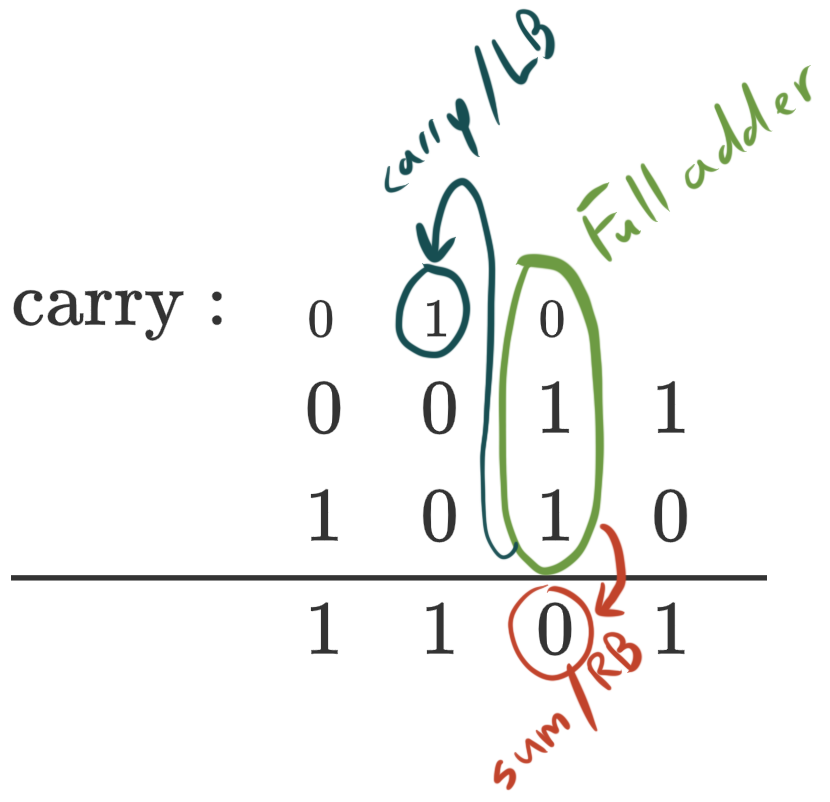
\includegraphics[width=0.3\linewidth]{./images/adders.png}
\end{center}

\begin{framed}
\textbf{Opdracht 3.6} 
Vind twee of drie andere groepjes en maak gezamenlijk een 4-bits optelschakeling met \textit{full adders}.\\
Zorg voor labeling van inputs, outputs en volgorde van de adders.\\

Teken het schema op je antwoordblad. Je mag een \textit{full adder} als een enkele module tekenen, met drie inputs en twee outputs. Als je dit doet, label de outputs van elke \textit{full adder} (\textit{sum} en \textit{carry}).\\

\textit{Let op: er kan overflow ontstaan. Zorg voor een vijfde output die overflow aangeeft.}
\end{framed}

\begin{framed}
\textbf{Aftekenen!} Laat opdracht 3.6 aftekenen.
\end{framed}

\newpage
\section*{Optel-/aftrekschakeling}

We bouwen nu een schakeling die zowel kan optellen als aftrekken met behulp van \textit{two's complement} representatie.

Bij \textit{two's complement} wordt aftrekken $A - B$ gerealiseerd door alle bits van B te flippen en vervolgens 1 op te tellen bij het eindresultaat. Oftewel, $A - B = A + \overline{B} + 1$, waarbij $\overline{B}$ wordt verkregen door alle bits van $B$ te flippen.

De bijkomende moeilijkheid is dat we de bits van $B$ alleen willen flippen als de $\textrm{SUB/}\overline{\textrm{ADD}}$ de waarde $1$ heeft, want dan willen we aftrekken. (Als de $\textrm{SUB/}\overline{\textrm{ADD}}$ de waarde $0$ heeft willen we optellen en moeten we de bits van $B$ dus niet flippen.)

Dit geeft de volgende waarheidstabel per bit van $B$:

\[
\begin{array}{cc|c}
\textrm{SUB/}\overline{\textrm{ADD}} & \textrm{Input bit} & \textrm{Output bit} \\
\hline
0 & 0 & 0 \\
0 & 1 & 1 \\
1 & 0 & 1 \\
1 & 1 & 0
\end{array}
\]

\begin{framed}
\textbf{Opdracht 3.7}
Met welke logische poort kun je deze waarheidstabel realiseren?
\end{framed}

\begin{framed}
\textbf{Opdracht 3.8}
Maak een 4-bits optel-/aftrekschakeling. De schakeling heeft 8 inputs en de $SUB/\overline{ADD}$-selectiebit.\\
Teken het schema op je antwoordblad.\\
\textit{Let op: de overflow mag bij deze schakeling worden genegeerd.}
\end{framed}

\begin{framed}
\textbf{Aftekenen!} Laat opdracht 3.7 en 3.8 aftekenen.
\end{framed}

\newpage 
\ 
\thispagestyle{empty}
\newpage
\raggedleft

\includegraphics[width=0.2\textwidth]{images/uvalogo_regular_compact_p_nl.eps}
\vfill
PIDAC\\
Minor Programmeren\\
Datarepresentaties, Tools en Technieken\\

\thispagestyle{empty}
\end{document}
